\section[Introduction]{Introduction}
\label{chap:introduction}
\epigraph{\centering \textit{“Things like chatbots, machine learning tools, natural language processing, or sentiment analysis are applications of artificial intelligence that may one day profoundly change how we think about and transact in travel and local experiences.”}}{Gillian Tans}

Sentiment Analysis or Opinion Mining is a way of finding out the polarity or strength of the opinion (positive or negative) that is expressed in written text \cite{samuels_news_2020}.\\
It is used in business to understand social sentiment for their brand, a particular product or service.

\subsection[Previous work]{Previous work}
\label{chap:previouswork}
In the last semester, my project partner and I have for the first time stepped into the world of sentiment analysis, making use of various supports such as tutorials, explanations, and lots of research.
We then decided to use all the material we had found to build something of our own, so we built a tool to categorize the sentiment of hotel reviews.
We wanted to split the sentiment of the reviews into 5 categories: from awful to excellent.
At the end of the project, we managed to have an \gls{accuracy} of about 0.48, taking into consideration the 5 categories was a good result.


\subsection[Project description]{Project description}
\label{chap:intropj_desc}
The thesis project I am working on this semester will still be on sentiment analysis. This time the model created will be used to make predictions about newspaper news, to understand the polarity (positive or negative) of an article or the newspaper itself.
A newspaper can change people's way of thinking and mood because of its polarity. That is why it is vital to understand its importance.
By having the polarity of a newspaper, I can also calculate a lot of things such as: the polarity of a newspaper over time, the various categories, and which of these newspapers affect us the most.

\subsection{Motivation}
As already mentioned, this technology allows to crystallize negative and positive feelings from a text. Besides sentiment classification, sentiment analysis brings many other benefits in areas such as marketing and customer satisfaction. Some of these benefits could be, for example:

\begin{itemize}
\item \textbf{Customer classification}\\
sentiment analysis allows customers to be classified according to their emotional mood. This offers the opportunity to find customers who are more willing to buy.
\item \textbf{Chatbot training}\\
With the results of the sentiment analysis tool, it is possible to train chatbots to recognize and respond to specific customer sentiments.
\item \textbf{Scalability and automation}\\
As a digital tool, sentiment analysis can be easily extended or integrated into an automated system.
\end{itemize}

From these points, a strongly increasing tendency regarding the application of sentiment analysis can be assumed. This makes it even more relevant for developers to get to grips with it. From the developer's perspective, learning sentiment analysis also promotes new experiences in areas such as: 

\begin{itemize}
\item Data analytics
\item Data science
\item Machine learning
\item Predictive modelling
\end{itemize}

\subsection[Goal]{Goal}
\label{chap:intro_goal}
The core of this project is with the help of different tools like \gls{Tensorflow} \cite{tensorflow}, \gls{Keras} \cite{noauthor_keras_nodate} and \gls{BERT} \cite{devlin_bert_2019} to create a model that takes text as input and classifies it in “positive” or “negative”. 
To calculate the polarity of the article, I will use different datasets to create different models, in the end I will use the model and dataset that most reflects my purpose.
Unfortunately, due to an impediment, my partner from the previous project was not able to take part in this assignment, which means that I must continue this project alone.
For a matter of timing and difficulty, I have resized the project and the categories on which to make a prediction will no more be 5 as in the last project, but 2.
This model should be available as a single component that can be integrated into arbitrary applications.\\
For the implementation of the project, I have used several websites and tutorials:
\begin{itemize}
    \item Tutorial for \gls{Keras} \cite{tutorial_keras}
    \item Deep-Learning-For-Hackers \cite{git}
    \item Sentiment Analysis with TensorFlow 2 and \gls{Keras} \cite{tutorial}
    \item Deep Learning LSTM for Sentiment Analysis \cite{karikari_deep_2020}
    \item Natural Language Processing and Sentiment Analysis using \gls{Tensorflow} \cite{khan_natural_2020}
    \item Sentiment Analysis: First Steps With Python's NLTK Library \cite{python_sentiment_nodate}
    \item Sentiment Analysis using Deep Learning with \gls{Tensorflow} \cite{pandey_sentiment_2020}
    \item Practical Text Classification With Python and \gls{Keras} \cite{python_practical_nodate}
    \item Classify text with \gls{BERT} \cite{noauthor_classify_nodate}
    \item Text Classification with \gls{BERT} using Transformers for long text inputs \cite{girdhar_text_2020}
    \item Simple Transformers — Multi-Class Text Classification with \gls{BERT}, RoBERTa, XLNet, XLM, and DistilBERT \cite{rajapakse_simple_2019}
    \item Fine-tuning \gls{BERT} with \gls{Keras} and tf.Module \cite{antyukhov_fine-tuning_2020},
    \item The 1cycle policy \cite{gugger_1cycle_nodate},
    \item \gls{Ktrain} tutorials \cite{maiya_amaiyaktrain_2021}.
\end{itemize}


\subsection{Project organization}
Table~\ref{tab:Organisation} describes who occupies which role in our project organization:
\begin{longtable}[ c ]{| m{5cm} | m{5cm}|  m{3cm}|}
 \hline
 \multicolumn{3}{| c |}{\textbf{Project organization}}\\
 \hline
 \textbf{Role in the \newline project organization} & \textbf{Name}  & \textbf{BFH\newline Abbreviation}\\
 \hline
 \endfirsthead
%
 \multicolumn{3}{c}%
 {{\bfseries Table \thetable\ continued from previous page}} \\
 \hline
 \textbf{Role in the \newline project organization} & \textbf{Name}  & \textbf{BFH Abbreviation}\\
 \hline
 \endhead
%
{Tutor}   & {Mascha Kurpicz-Briki}  & {kim3}   \\ \hline
{Expert}  & {Andreas Dürsteler}         & {-}   \\ \hline
{Developer}     & {Giorgio Bakhiet Derias}& {bakhg1}\\ \hline
                 
\caption{Project organization}
\label{tab:Organisation}\\
\end{longtable}

\subsection{Tools}
\label{chap:intro_tools}
In Table~\ref{tab:Tools} is possible to find the different tools I used for this project:
\begin{longtable}[ c ]{| m{4cm} | m{10cm}|}
 \hline
 \multicolumn{2}{| c |}{\textbf{Tools}}\\
 \hline
 \textbf{Tool}  & \textbf{Description}\\
 \hline
 \endfirsthead
%
 \multicolumn{2}{c}%
 {{\bfseries Table \thetable\ continued from previous page}} \\
 \hline
\textbf{Tool}  & \textbf{Description}\\
 \hline
 \endhead
%
{\gls{jupyter}}           & {A document that can store code, diagrams, graphics and much more.}      \\ \hline
{Google   \gls{colab}oratory} & {Online platform to host \gls{jupyter}.} \\ \hline
{\gls{kaggle}}   & {Is an online machine learning environment and community.}      \\ \hline  
{\gls{anaconda}}          & {Application to manage libraries of larger projects.}      \\ \hline
{\gls{virtual machine}}   & {\gls{anaconda} is installed on the virtual machine to run the project.}      \\ \hline
{PyCharm}   & {IDE used for the Python language. It is developed by the company JetBrains.}      \\ \hline
{GitHub}   & {GitHub is a hosting service for software projects.}      \\ \hline
{\gls{Overleaf}}   & {\gls{Overleaf} is a cloud-based collaborative LaTeX editor used to write, edit, and publish scientific papers.}      \\ \hline
{\gls{MLMP}}   & {\gls{MLMP} is a cloud-based environment for machine learning created by BFH.}      \\ \hline
{\gls{Scikit-learn}}           & {Open-source machine learning software library for the Python programming language.}      \\ \hline
{\gls{Tensorflow}}   & {Open-source software library for machine learning.}      \\ \hline
{\gls{Pandas}}   & {Open-source data analysis and tool for data manipulation, built in Python.}      \\ \hline
{\gls{Keras}}             & {\gls{Tensorflow} library specifically for creating neural networks.}      \\ \hline
{\gls{Ktrain}}   & {\gls{Ktrain} is a library used to build, train, debug, and deploy neural networks in the deep learning software framework \gls{Keras}.}      \\ \hline
{\gls{BERT}}   & {Is a recent paper published by researchers at Google AI Language.}      \\ \hline
{\gls{Hugging Face}}   & {Is an open-source provider of natural language processing (NLP) technologies.} \\ \hline
{\gls{Plotly}}   & {\gls{Plotly} provides online graphing, analytics, and statistics tools for individuals and collaboration, and libraries for Python, R, MATLAB, Perl, Julia, Arduino, and REST.}   \\ \hline

 

\caption{Tools}
\label{tab:Tools}\\
\end{longtable}

\subsection{Project pipeline}
The Project pipeline is shown in Figure~\ref{fig:fig_pipeline}, the pipeline goes from top to bottom.
The pipeline is categorized by color, in fact each color is a key component of the project:
\begin{itemize}
    \item in orange there is the part that concerns the creation of the dataset (Chap:\ref{chap:dataset},\ref{chap:work on dataset}),
    \item in red the part related to \gls{Ktrain} (Chap:\ref{chap:Ktrain model}),
    \item orange and red together will create the model (Chap:\ref{chap:model training}),
    \item in green the data coming from the APIs, this data will be given to the trained model to make predictions (Chap:\ref{chap:model test newspaper}),
    \item in blue the components related to the calculation of polarity, analysis of results and creation of visualization (Chap:\ref{chap:model plot}). 
\end{itemize}
  
\begin{figure}[ht!]
\centering
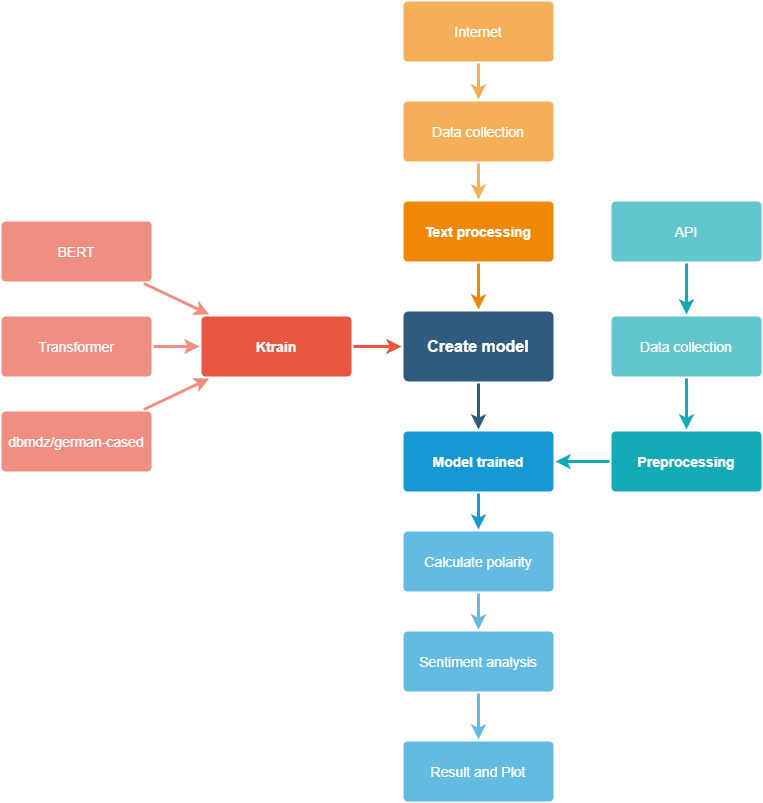
\includegraphics[width=0.9\textwidth]{images/test1.png}
\caption{Project pipeline}
\label{fig:fig_pipeline}
\end{figure}
\FloatBarrier